\documentclass{standalone}
\usepackage{tikz}
\begin{document}
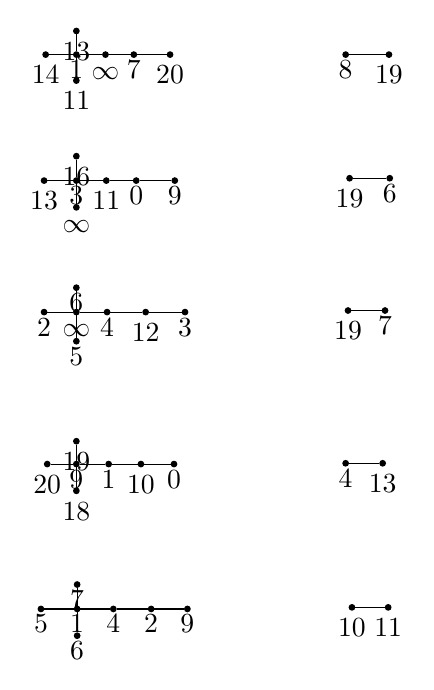
\begin{tikzpicture}[every node/.style={draw, circle, fill=black, minimum size=2pt, inner sep=0pt}]
\node[fill=black, label=below:{\color{black}$14$}] (G1N14) at (2.31,7.51) {};
\node[fill=black, label=below:{\color{black}$1$}] (G1N1) at (2.70,7.51) {};
\node[fill=black, label=below:{\color{black}$\infty$}] (G1Ninf) at (3.07,7.51) {};
\node[fill=black, label=below:{\color{black}$7$}] (G1N7) at (3.43,7.51) {};
\node[fill=black, label=below:{\color{black}$20$}] (G1N20) at (3.89,7.51) {};
\node[fill=black, label=below:{\color{black}$11$}] (G1N11) at (2.70,7.18) {};
\node[fill=black, label=below:{\color{black}$13$}] (G1N13) at (2.70,7.81) {};
\node[fill=black, label=below:{\color{black}$8$}] (G1N8) at (6.12,7.51) {};
\node[fill=black, label=below:{\color{black}$19$}] (G1N19) at (6.67,7.51) {};
\draw (G1N1) -- (G1N14);
\draw (G1N1) -- (G1N11);
\draw (G1N1) -- (G1N13);
\draw (G1N1) -- (G1Ninf);
\draw (G1Ninf) -- (G1N7);
\draw (G1N20) -- (G1N7);
\draw (G1N8) -- (G1N19);
\node[fill=black, label=below:{\color{black}$13$}] (G2N13) at (2.29,5.91) {};
\node[fill=black, label=below:{\color{black}$3$}] (G2N3) at (2.70,5.91) {};
\node[fill=black, label=below:{\color{black}$11$}] (G2N11) at (3.08,5.91) {};
\node[fill=black, label=below:{\color{black}$0$}] (G2N0) at (3.46,5.91) {};
\node[fill=black, label=below:{\color{black}$9$}] (G2N9) at (3.95,5.91) {};
\node[fill=black, label=below:{\color{black}$\infty$}] (G2Ninf) at (2.70,5.57) {};
\node[fill=black, label=below:{\color{black}$16$}] (G2N16) at (2.70,6.22) {};
\node[fill=black, label=below:{\color{black}$19$}] (G2N19) at (6.17,5.94) {};
\node[fill=black, label=below:{\color{black}$6$}] (G2N6) at (6.68,5.94) {};
\draw (G2N3) -- (G2N13);
\draw (G2N3) -- (G2Ninf);
\draw (G2N3) -- (G2N16);
\draw (G2N3) -- (G2N11);
\draw (G2N11) -- (G2N0);
\draw (G2N9) -- (G2N0);
\draw (G2N6) -- (G2N19);
\node[fill=black, label=below:{\color{black}$2$}] (G3N2) at (2.29,4.24) {};
\node[fill=black, label=below:{\color{black}$\infty$}] (G3Ninf) at (2.70,4.24) {};
\node[fill=black, label=below:{\color{black}$4$}] (G3N4) at (3.09,4.24) {};
\node[fill=black, label=below:{\color{black}$12$}] (G3N12) at (3.58,4.24) {};
\node[fill=black, label=below:{\color{black}$3$}] (G3N3) at (4.08,4.24) {};
\node[fill=black, label=below:{\color{black}$5$}] (G3N5) at (2.70,3.87) {};
\node[fill=black, label=below:{\color{black}$6$}] (G3N6) at (2.70,4.55) {};
\node[fill=black, label=below:{\color{black}$19$}] (G3N19) at (6.15,4.26) {};
\node[fill=black, label=below:{\color{black}$7$}] (G3N7) at (6.62,4.26) {};
\draw (G3Ninf) -- (G3N2);
\draw (G3Ninf) -- (G3N5);
\draw (G3Ninf) -- (G3N6);
\draw (G3Ninf) -- (G3N4);
\draw (G3N4) -- (G3N12);
\draw (G3N3) -- (G3N12);
\draw (G3N7) -- (G3N19);
\node[fill=black, label=below:{\color{black}$20$}] (G4N20) at (2.33,2.31) {};
\node[fill=black, label=below:{\color{black}$9$}] (G4N9) at (2.70,2.31) {};
\node[fill=black, label=below:{\color{black}$1$}] (G4N1) at (3.11,2.31) {};
\node[fill=black, label=below:{\color{black}$10$}] (G4N10) at (3.52,2.31) {};
\node[fill=black, label=below:{\color{black}$0$}] (G4N0) at (3.94,2.31) {};
\node[fill=black, label=below:{\color{black}$18$}] (G4N18) at (2.70,1.97) {};
\node[fill=black, label=below:{\color{black}$19$}] (G4N19) at (2.70,2.60) {};
\node[fill=black, label=below:{\color{black}$4$}] (G4N4) at (6.12,2.32) {};
\node[fill=black, label=below:{\color{black}$13$}] (G4N13) at (6.59,2.32) {};
\draw (G4N9) -- (G4N20);
\draw (G4N9) -- (G4N18);
\draw (G4N9) -- (G4N19);
\draw (G4N9) -- (G4N1);
\draw (G4N1) -- (G4N10);
\draw (G4N0) -- (G4N10);
\draw (G4N4) -- (G4N13);
\node[fill=black, label=below:{\color{black}$5$}] (G5N5) at (2.25,0.47) {};
\node[fill=black, label=below:{\color{black}$1$}] (G5N1) at (2.71,0.47) {};
\node[fill=black, label=below:{\color{black}$4$}] (G5N4) at (3.17,0.47) {};
\node[fill=black, label=below:{\color{black}$2$}] (G5N2) at (3.65,0.47) {};
\node[fill=black, label=below:{\color{black}$9$}] (G5N9) at (4.11,0.47) {};
\node[fill=black, label=below:{\color{black}$6$}] (G5N6) at (2.71,0.13) {};
\node[fill=black, label=below:{\color{black}$7$}] (G5N7) at (2.71,0.78) {};
\node[fill=black, label=below:{\color{black}$10$}] (G5N10) at (6.20,0.49) {};
\node[fill=black, label=below:{\color{black}$11$}] (G5N11) at (6.66,0.49) {};
\draw (G5N1) -- (G5N5);
\draw (G5N1) -- (G5N6);
\draw (G5N1) -- (G5N7);
\draw (G5N1) -- (G5N4);
\draw (G5N4) -- (G5N2);
\draw (G5N9) -- (G5N2);
\draw (G5N11) -- (G5N10);
\end{tikzpicture}
\end{document}
